\documentclass[../languages.tex]{subfiles}

\begin{document}
\usec{C++}\label{sec:c__}

\cd{C++} is a general-purpose programming languages. It has imperative,
object-oriented and generic programming features, while also providing
facilities for low-level memory manipulation.

It was designed with a bias toward system programming and embedded,
resource-contained and large systems, with performance efficiency and
flexibility to use as its design highlights. \cd{C++} has also been found
useful in many other contexts, with key strengths being software infrastructure
and resource constrained applications, including desktop applications, servers
(e.g.\ e-commerce, web search, or SQL servers), and performance-critical
applications (e.g.\ telephone switches or space probes). \cd{C++} is a compiled
languages, with implementations of it available on many platforms.  Many
vendors provide \cd{C++} compilers, including the Free Software Foundation,
Microsoft, Intel, and IBM.

\cd{C++} is standardized by the International Organization for Standardization
(ISO), with the latest standard version ratified and published by ISO in
December 2017 as ISO/IEC 14882:2017 (informally known as \cd{C++17}). The
\cd{C++} programming languages was initially standardized in 1998 as ISO/IEC
14882:1998, which was then amended by the \cd{C++03}, \cd{C++11}, and
\cd{C++14} standards. The current \cd{C++17} standard supersedes these with new
features and an enlarged standard library. Before the initial standardization
in 1998, \cd{C++} was developed by Bjarne Stroustrup at Bell Labs since 1979,
as an extension of the \cd{C} languages as he wanted an efficient and
flexible language similar to \cd{C} which also provided high-level features for
program organization.  \cd{C++20} is the next planned standard thereafter.

Many other programming languages have been influenced by \cd{C++}, including
\cd{C\#}, \cd{D}, \cd{Java}, and newer versions of \cd{C}.

\subsection{Influence}
\label{sub:influence}

\begin{Figure}
  \centering
  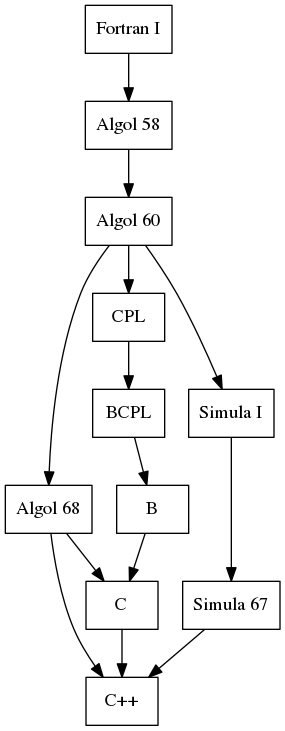
\includegraphics[height=0.5\textheight]{cpp}
  \captionof{figure}{Inheritance diagram for \cd{C++}.}
\end{Figure}

\cd{C++} was primarily influenced by the languages \cd{Ada}, \cd{Algol},
\cd{C}, \cd{CLU}, \cd{ML}, \cd{Simula}, and \cd{Python}.

\subsection{Hello World}
\label{sub:hello_world}

\begin{minted}[frame=lines]{cpp}
#include <iostream>

int main() {
  std::cout << "Hello, world!\n";
}
\end{minted}

\subsection{Syntax}\label{sub:syntax}

\newpage
\end{document}
